%Chapter of Background
%Take everything from poster and then add a whole lot
%Explain AE,signing,cipers, types of attack that my app may have to defend against, keys, nonces, 

\chapter{Background}
\label{back}

\section{Cryptography}

Cryptography is the practise and study of techniques for secure communication in the presence of attackers. To do so, one can use encryption where by messages are encoded in such a way that only authorised parties, or at least parties in possession of the keys, can view them. There are two main ways of encryption Symmetric Key encryption and Asymmetric Key encryption. In Symmetric Key encryption both parties have the same key which can encrypt and decrypt messages that are sent between them. The problem is that if Bob wants to send an encrypted message to Alice, he must get the secret key to her. Currently the most secure way for the transmission of secret keys is to hand them over in person, in private. This this project Asymmetric Key encryption and Digital signatures.


\subsection{Asymmetric Key Encryption}

To get round the problem of secure sending of secret keys, one can use Asymmetric Key encryption which involves a secret key and a public key, the public key is generated out of the secret key and are therefore mathematically linked but it is computationally infeasible to calculate the secret key from the public key. This public key can be given out freely and is not a secret. So if Bob sends a message to Alice he encrypts the message with her public key and she can decrypt it with her secret key. This type of key encryption gets past the sharing secret key problem, as long as you can make sure the public key is indeed the correct one, but it only stops attackers from reading the message. It does not prove the message was sent by a certain person or that the message has not been altered in transit.

\begin{figure}[H]
	\centering
	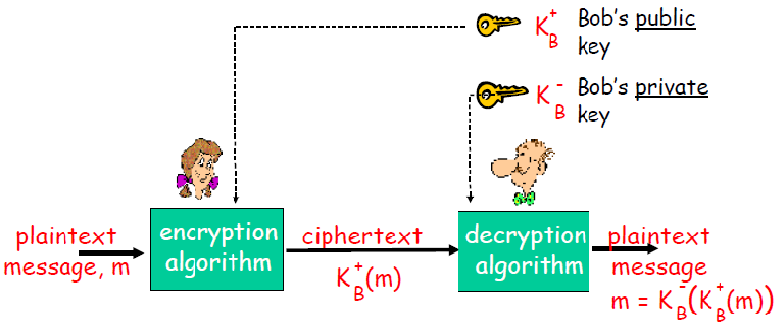
\includegraphics[width=1\linewidth]{Figures/publickeyex.png}
	\caption{Asymmetric Key Encryption}
	\label{fig:asy}
\end{figure}


\subsection{Stream Cipher}

A stream cipher is a symmetric key cipher where the plain text message is combined with a cipher digit stream so that each digit of the plain text is encrypted individually. The combining operation is an XOR.

\subsection{Digital Signature}

This is a mathematical scheme for proving message authenticity, message integrity and message non-repudiation. Similarly to asymmetric key encryption a random private key is created with a corresponding public key. The algorithm takes in a message and a private key and using SHA-512, it creates a hash using the private key and message. It then appends that signature to the message. If Alice signs a message in this way, Bob can use another algorithm to verify the message with the public key and signature. It is important to note that the data is not hidden at this point, it is still in plain text.

\subsection{Message Authentication Code}

A MAC is a small piece of information that is used to authenticate a message and prove it's integrity. The MAC algorithm takes in a message and a key and produces a MAC, then it is sent with the message and the receiver runs the algorithm like the sender and if the resulting MAC is the same as the received MAC then the message has not been altered. MACs differs to digital signatures in that it does not provide message repudiation.

\section{TweetNaCl}

NaCl or ``Salt`` is a simple to use high-speed library for authenticated encryption. It provides both Asymmetric and Symmetric encryption, authentication and message integrity with SHA-512. The authors are Daniel J. Bernstein, Tanja Lange and Peter Schwabe but at points it does rely on third part implementations for parts. The API is simple, having only a handful of methods but uses high speed, high security primitives\cite{naclsmall}.

It provides everything needed for secure data transmission but unfortunately the library is relatively quite large, the Arduino Due has at it's disposal 512KB flash memory and the full library is 3MB. Fortunately the same creators along with Bernard van Gastel, Wesley Janssen and Sjaak Smetsers made TweetNaCl. Which is a tiny implementation of NaCl, still providing speed and security but with a significantly smaller code size 40KB. It retains the same protections against timing attacks, cache-timing attacks, has to branches depending on secret data and no array indices depending on secret data. In addition it is thread-safe and has no dynamic memory allocation\cite{tweetnacl}. It is portable and easy to integrate, the library is easily added as it consists of two files, there is no complicated configuration to be set up or any dependencies on external libraries. Because of this compactness it is easier to read and understand it's operation. Although not as fast as NaCl it is still fast enough for most applications. The authors of the library feel that the performance is acceptable as``Most applications can tolerate the 4.2 million cycles that OpenSSL uses on an Ivy Bridge CPU for RSA-2048 decryption, for example, so they can certainly tolerate the 2.5 million cycles that TweetNaCl uses for higher-security decryption (Curve25519).'' \cite{tweetnacl3}.

TweetNaCl is still small after compilation at 11KB thus avoiding instruction cache misses. It is a full library and not a set of isolated functions, for a TweetNaCl application, only six functions are needed. crypto\_box for public-key authenticated encryption; crypto\_box\_open for ecryption; crypto\_box\_keypair to create a encryption key pair; and similarly for signature keypairs crypto\_sign\_keypair, to sign messages crypto\_sign and to verify signatures crypto\_sign\_open, and. It is open source and the developers encourage it to be used as much as possible. 

Unfortunately the library won't compile as is on a Arduino, one problem is that there is no /dev/random and therefore no randombytes() which means that it can't create truly random secret keys and therefore good keypairs. The Arduinos can generate pseudorandom numbers by generating a seed from an analogue pin which will provide fairly random numbers but it is considered insecure for cryptographic applications to use pseudorandom numbers\cite{arduinopseudo}. It is possible to create true random numbers by utilising the truly random nature of atmospheric noise or background radiation but this requires extra components and is outside the scope of this project. 

Also, as mentioned in the implementation the Arduino can't use the C library as is, it needs to be converted into a C++ header file and cpp file relationship.

For public key authenticated encryption, TweetNaCl uses three components: Curve25519 Diffie–Hellman key-exchange function, Salsa20 stream cipher for message encryption and Poly1305 for message authentication. 

Curve25519 Diffie–Hellman key-exchange function is used to compute the shared secret between sender and receiver using the sender's secret key and receivers public key. Curve25519 is an elliptic curve, which is an approach to public key cryptography that is based on the algebraic structure of elliptic curves over finite fields, used in conjunction with the elliptic curve Diffie-Hellman anonymous key agreement protocol\cite{curve}

For message encryption the Salsa20 stream cipher encrypts a message using the shared secret. Salsa20 uses a pseudorandom function based on add-rotate-xor, bitwise additions and rotation operations. The cipher uses XOR operations, 32-bit addition mod $2^{32}$ and constant-distance rotation operations on an internal state of sixteen 32-bit words\cite{salsa}.

The library uses Poly1305 as it's MAC function. In TweetNaCl, Poly1305 as it uses the Salsa20 stream cipher to compute the code\cite{poly}.

For key signature, TweetNaCl has a fourth component, Ed25519 public key signature system. Edwards curve digital signature algorithm is a variant of Schnorr signature based on Twisted Edward curves. It is faster than existing schemes but does not reduce strength of security\cite{ed25}. TweetNaCl gets it's name because the developers tweeted all of the source code in a 100 tweets to prove how small it was.

%explain how the encryption and signature's work. high level overview
% Curve25519 Diffie–Hellman key-exchange function public key
% Ed25519 signature 

\section{Types of attacks}

\subsection{Replay Attack}
When this attack occurs when the attacker replays a valid message. If Bob wants Alice to prove who she and she duly provides some encrypted signature to prove so. Eve can capture that signature, She does not know what the signature is but she knows that it is a signature. She can then connect to Bob and use this message to pretend she is Alice. To prevent this attack Alice might use an identifier that is only valid for one use, this could be session tokens or a one-time passwords. 

\subsection{Man in the Middle Attack}
In this attack there is an attacker between two parties, Bob and Alice, who wish to communicate. The man in the middle, Eve, changes messages as they are in transit and manages to pretend that she is the person that the other thinks they are talking to. An example is if Alice asks for Bob's public key, Eve can capture that public key, replace it with her own and send that and because Alice has no way to prove that it is Bob's key or not she accepts it. So when Alice sends a message that has been encrypted with what she thinks is Bob's key, Eve can take it, decrypt it with her key, change the message then encrypt it with Bob's real public key. Which Bob receives and believes the message is from Alice.

\subsection{Bit-Flipping Attack}
This is where the attacker can change the cipher text in some way that causes a predictable change in the plain text. Eve does not need to know exactly what the plain text is. For example if Alice was to send a message to Bob saying that she owes him £100 and Eve knows at least some of the message format, she can change the number at the end into £1000. 

\subsection{Stream Cipher Attack}
If the same key is reused in a stream cipher then it becomes vulnerable. If Alice were to encrypt two messages of the same length with the same key, Eve can take the two encrypted messages and XOR them to produce A XOR B and thus find the message. If one message was longer than the other then Eve could only find out the section of the longer message that was the same length as the shorter.

\section{Timing Attack}
In this type of attack strategy, an attacker measures the time that the legitimate user takes to perform some action that involves the secret key. If the time taken depends on the key then it is possible to deduce information about the key. For example the login program in early versions of Unix executed the crypt function only when the login name was recognised. By this an attacker was able to find out if a login name was correct even if the password wasn't.

\section{Machine to Machine}

M2M refers to the direct communication between two devices using any sort of channel. This is a component of IoT and when connected in this way small, low power sensors can transmit their data to another device which can collate, perform analysis or some extra computation or pass the data along again before it reaches a human user. Present day applications include monitoring the health of machinery, digital billboards or sensory networks. An application may possess multiple sensors in a network that pass sensor data to multiple nodes which do some computation, such as adjust machines to correct errors, replenish stock or manage a system and possibly sending information, such as state across the Internet to a human user.

\section{Technologies used}

In this project the Arduino was programmed using C++. The C++ was developed in the Arduino IDE. An Arduino Due, Arduino Uno, DS1820S temperature sensor, resistor and two Ethernet Shield R2 boards were used. On the server side there is an SQL server, PHP scripts that accept that Arduino data and put it in the SQL server. And a Java web application that uses Java Database Connectivity, JBCD, to access the SQL server and outputs dynamic HTML when accessed. The Java code was developed using Eclipse Jee Mars. Bitbucket, in conjunction with Git, was used to remotely store all the software.

\subsection{XAMPP Server}

XAMPP, Apache, MySQL, PHP and Perl come together to form XAMPP which is free, open source, cross platform, web server stack package for the creation and testing of local server systems that can then be moved as they are onto live systems. This XAMPP used in this project also contains Tomcat.

\subsection{PHP}
PHP is a server-side scripting language used in web development. It is especially suited server-side applications as it is very portable. PHP code in a file that is requested is executed by the PHP runtime. It can be used with many OS's, web serves and relational database management systems. It is very common for web hosting providers to support PHP use by their clients.

\subsection{SQL}

Standard Query Language is a special purpose programming language for managing data store in relational databases. SQL organises data into databases and tables and has operations for inserting, updating, deleting, altering and querying data. The vast majority of the databases use SQL.

\subsection{Apache Tomcat}

Tomcat is an open source implementation of the Java servlet, JavaServer Pages, Java Expression Language and Java Websocket technologies. It provides the ability to produce dynamic HTML in a pure Java environment. It accepts web application archives, WAR, files for ease of updating web apps.

%JBCD? Accessible through web by port forwarding.
\section{Secure Transmission of Keys}

The problem is more acute with symmetric key encryption as it is the same key used to encrypt and decrypt a message, if the key is compromised messages can no longer be trusted. The most secure and high tech solution is to meet in person and in private with the person you plan to communicate with and exchange keys there. If the communication is of a diplomatic nature, the bag used to transport the keys can have special legal protection against being opened and this is called a diplomatic bag\cite{dipbag}. You could send a key over a another secure channel that you trust but there is always the chance that it has been compromised and it is not possible to verify that the person on the other side of the secure channel is who you think it is without first having a secure identifier which you can't get solely through internet communication. There is a similar problem with Asymmetric key encryption, a user can freely distribute their public key and they can be pretty sure that the messages they receive are secure but it is not possible to prove who has sent you the message without their public key signature but initially public key transmission is vulnerable to man in the middle attacks.
